% !TeX recipe = Tectonic
% CV - Marko Rosic - tailored for Canonical, Senior Design Manager (Infrastructure)
% Compile with: cd applications/canonical && tectonic Marko_Rosic_CV.tex
\documentclass[a4paper,9.5pt]{article}

% ── Font ──────────────────────────────────────────────────────────────
\usepackage{fontspec}
\setmainfont{Fira Sans}[
  BoldFont       = {Fira Sans Bold},
  ItalicFont     = {Fira Sans Italic},
  BoldItalicFont = {Fira Sans Bold Italic}
]
\newfontfamily\symfont{Zapf Dingbats}

% ── Layout ────────────────────────────────────────────────────────────
\usepackage[a4paper, top=1.5cm, bottom=1.4cm, left=1.8cm, right=1.8cm]{geometry}
\usepackage{microtype}
\usepackage{needspace}

% ── Colors ────────────────────────────────────────────────────────────
\usepackage{xcolor}
\definecolor{darktext}{HTML}{111111}
\definecolor{midgray}{HTML}{555555}
\definecolor{lightgray}{HTML}{999999}
\definecolor{hairline}{HTML}{BBBBBB}

% ── Links ─────────────────────────────────────────────────────────────
\usepackage[hidelinks]{hyperref}
\urlstyle{same}
\usepackage[normalem]{ulem}

% ── Lists ─────────────────────────────────────────────────────────────
\usepackage{enumitem}

% ── Tables ────────────────────────────────────────────────────────────
\usepackage{array}

% ── TikZ ──────────────────────────────────────────────────────────────
\usepackage{tikz}
\usetikzlibrary{calc}

% ── Section headings ──────────────────────────────────────────────────
\usepackage{titlesec}
\titleformat{\section}
  {\normalfont\small\bfseries}
  {}{0em}{\MakeUppercase}
  [\vspace{3pt}{\color{darktext}\hrule height 0.4pt}]
\titlespacing*{\section}{0pt}{22pt}{12pt}

% ── Page style ────────────────────────────────────────────────────────
\pagestyle{empty}
\setlength{\parindent}{0pt}
\setlength{\parskip}{0pt}

% ── Column dimensions ─────────────────────────────────────────────────
\newlength{\cvdatecol}  \setlength{\cvdatecol}{2.5cm}
\newlength{\cvsymcol}   \setlength{\cvsymcol}{1cm}
\newlength{\cvcontcol}  \setlength{\cvcontcol}{\dimexpr\textwidth-\cvdatecol-\cvsymcol\relax}

% ── Symbol counter ────────────────────────────────────────────────────
\newcounter{cvsymn}
\newif\ifcvfirst\cvfirsttrue

% ── TikZ asterisk with named remember-picture node ───────────────────
\newcommand{\cvastsym}{%
  \begin{tikzpicture}[remember picture, baseline=(sym-\thecvsymn.base)]
    \node[inner sep=0pt, outer sep=0pt, text=darktext, font=\normalsize\symfont] (sym-\thecvsymn) {✱};
  \end{tikzpicture}%
}

% ── Portfolio button ──────────────────────────────────────────────────
\newcommand{\portfoliobutton}{%
  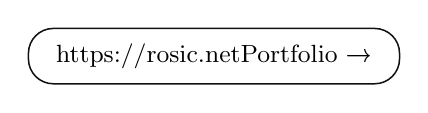
\begin{tikzpicture}[baseline=(btn.base)]
    \node[draw=darktext, rounded corners=9pt,
          inner xsep=10pt, inner ysep=5.5pt,
          line width=0.55pt, font=\small,
          outer sep=0pt] (btn)
      {\href{https://rosic.net}{Portfolio~→}};
  \end{tikzpicture}%
}

% ── Connector: hairline from prev asterisk to current, same page only ─
\newdimen\cvyprev
\newdimen\cvycurr
\newcommand{\cvdrawconnect}{%
  \edef\prevn{\the\numexpr\value{cvsymn}-1\relax}%
  \begin{tikzpicture}[overlay, remember picture]
    \coordinate (cvprev) at (sym-\prevn.center);
    \coordinate (cvcurr) at (sym-\thecvsymn.center);
    \pgfextracty{\cvyprev}{\pgfpointanchor{cvprev}{center}}%
    \pgfextracty{\cvycurr}{\pgfpointanchor{cvcurr}{center}}%
    \ifdim\cvyprev>\cvycurr%
      \draw[line width=0.35pt, color=hairline]
        ($(sym-\prevn)+(0,-4.5pt)$) -- ($(sym-\thecvsymn)+(0,4.5pt)$);%
    \fi%
  \end{tikzpicture}%
}

% ── Entry without company note ────────────────────────────────────────
\newcommand{\cventry}[3]{%
  \stepcounter{cvsymn}%
  \par\vspace{13pt}%
  \noindent%
  \makebox[\cvdatecol][r]{\small\bfseries\color{midgray}#1}%
  \makebox[\cvsymcol][c]{\cvastsym}%
  \parbox[t]{\cvcontcol}{%
    {\bfseries #2}\\[2.5pt]
    {\small#3}%
  }%
  \ifcvfirst\cvfirstfalse\else\cvdrawconnect\fi%
  \par%
}

% ── Entry with italic company context line ────────────────────────────
\newcommand{\cventrynote}[4]{%
  \stepcounter{cvsymn}%
  \par\vspace{13pt}%
  \noindent%
  \makebox[\cvdatecol][r]{\small\bfseries\color{midgray}#1}%
  \makebox[\cvsymcol][c]{\cvastsym}%
  \parbox[t]{\cvcontcol}{%
    {\bfseries #2}\\[2.5pt]
    {\small#3}\\[2.5pt]
    {\footnotesize\itshape\color{lightgray}#4}%
  }%
  \ifcvfirst\cvfirstfalse\else\cvdrawconnect\fi%
  \par%
}

% ── Bullet list ───────────────────────────────────────────────────────
\newenvironment{cvitems}{%
  \vspace{1pt}%
  \begin{itemize}[
    leftmargin = \dimexpr\cvdatecol+\cvsymcol+0.55em\relax,
    label      = {•},
    topsep     = 4pt,
    itemsep    = 3pt,
    parsep     = 0pt,
    partopsep  = 0pt
  ]\small\interlinepenalty=10000%
}{\end{itemize}}

% ── Skill block ───────────────────────────────────────────────────────
\newcommand{\skillblock}[2]{%
  {\small\bfseries #1}\newline%
  {\small\color{midgray}#2}%
}

% ══════════════════════════════════════════════════════════════════════
\begin{document}
% ══════════════════════════════════════════════════════════════════════

% ── HEADER ────────────────────────────────────────────────────────────
\vspace*{-0.3cm}
\noindent{\fontsize{30}{36}\selectfont\bfseries Marko Rosić}%
\hfill\makebox[0pt][r]{\portfoliobutton\hspace{2pt}}
\par\vspace{3pt}
{\small\color{midgray}%
  Cara Du\v{s}ana 118, Belgrade, Serbia~\textbar~%
  +381 60 585 44 55~\textbar~%
  \href{mailto:marko@rosic.net}{\uline{marko@rosic.net}}~\textbar~%
  \href{https://rosic.net}{\uline{rosic.net}}%
}

% ── SUMMARY ───────────────────────────────────────────────────────────
\section{Summary}

{\small Design manager with 15+ years building design systems and
leading teams at the intersection of design and engineering. I set
direction and quality standards, coach designers working on technically
complex products, and build the practices that connect design to how
engineering ships. My experience spans consumer products, carrier-branded
mobile applications, and backend operational tooling. I work remotely
in EMEA, use AI including Claude Code to build faster, and contribute
to open source tooling through Figma plugin development.}

% ── EXPERIENCE ────────────────────────────────────────────────────────
\section{Experience}

\cventry{5/2025\,--\,Present}{Design Leadership Consultant}{%
  Beyond Clicks Studio (Independent) \textbar{} Belgrade, Serbia (Remote)}
\begin{cvitems}
  \item Architected a multi-product design system end to end: defined
        token architecture, established component conventions, and built
        a Figma-variables-to-theme-tokens pipeline as a single source of
        truth across design and engineering
  \item Built Figma plugins to automate repetitive design tasks, reducing
        production time and closing the gap between design intent and
        engineering output
  \item Built AI-orchestrated workflows and internal tooling using Claude
        Code, owning the problem, the UX, and the research direction
  \item Directed UX end to end for a US youth-sports communication
        platform, from discovery through implementation oversight
\end{cvitems}

\cventrynote{7/2024\,--\,5/2025}{Head of UX/UI}{%
  Gentoo Media \textbar{} Belgrade, Serbia}{%
  Established following GiG Media's acquisition of Catena Media and
  subsequent spin-off of its media division.}
\begin{cvitems}
  \item Set design direction and standards across multi-brand products
        through a company-wide design system: token architecture,
        component conventions, and engineering handoff
  \item Led a design team of seven, managing and growing two team leads
        who each ran their own sub-team
  \item Changed how design and engineering collaborated, cutting
        time-to-market for new features by 25\%
  \item Used analytics and user feedback continuously to improve product
        quality
\end{cvitems}

\cventry{5/2021\,--\,7/2024}{Lead UX/UI Designer}{%
  Catena Media (acquired by GiG Media in 2023) \textbar{} Belgrade, Serbia}
\begin{cvitems}
  \item Built a design system for the flagship product that cut
        development time by 30\%, then scaled it across 10+ websites
  \item Ran workshops with product and engineering stakeholders to align
        design decisions with business goals
  \item Mentored junior designers and grew a team that worked well without
        hand-holding
\end{cvitems}

\cventry{10/2018\,--\,5/2021}{Senior UX/UI Designer}{%
  Catena Media \textbar{} Belgrade, Serbia}
\begin{cvitems}
  \item Led the redesign of the flagship product: mobile traffic up 20\%,
        user retention up 15\%
  \item Brought UX research and A/B testing into the product process,
        moving the team to evidence-based decisions
  \item Drove the migration from Sketch to Figma, improving how designers
        and engineers worked together
\end{cvitems}

\needspace{5\baselineskip}
\cventry{12/2013\,--\,10/2018}{Interaction Designer}{%
  Smith Micro Software, Inc \textbar{} Belgrade, Serbia}
\begin{cvitems}
  \item Designed UX for carrier-branded Android applications shipped with
        Sprint and T-Mobile devices: Visual Voicemail, messaging apps, and
        device companion tools
  \item Designed backend tooling for device management systems and an IoT
        location-based notification service, working at the boundary
        between consumer-facing UX and complex operational interfaces
  \item Collaborated directly with engineering across multiple carrier
        variants, meeting precise technical and brand specifications
\end{cvitems}

\cventry{2009\,--\,2013}{UI Designer}{%
  MySkin, Youngculture \textbar{} Belgrade, Serbia}
\begin{cvitems}
  \item Designed digital products and interfaces across client projects
\end{cvitems}

\cventry{2005\,--\,2008}{Co-founder \& CEO}{%
  Mainstream d.o.o. \textbar{} Belgrade, Serbia}
\begin{cvitems}
  \item Co-founded a dial-up ISP; led operations, finance, and product
        during the founding phase; the company later evolved into managed
        hosting and cloud services
\end{cvitems}

% ── SKILLS ────────────────────────────────────────────────────────────
\section{Skills}

\vspace{2pt}
\noindent
\begin{minipage}[t]{0.475\textwidth}
  \skillblock{Design Systems \& DesignOps}{%
    Token architecture, component libraries,
    design-engineering handoff,
    Figma (+ plugin development),
    Axure RP, HTML/CSS/JS prototyping}

  \vspace{12pt}
  \skillblock{Research \& Optimisation}{%
    User research \& usability testing,
    A/B testing, Google Analytics,
    VWO, HotJar, UXtweak}
\end{minipage}%
\hspace{0.05\textwidth}%
\begin{minipage}[t]{0.475\textwidth}
  \skillblock{Leadership \& Management}{%
    Design team management \& mentoring,
    Cross-functional stakeholder management,
    Design ops, roadmap planning,
    Jira, Asana, Linear, Notion}

  \vspace{12pt}
  \skillblock{Technical}{%
    HTML/CSS, JavaScript, PHP,
    Figma plugin development,
    Dev complexity assessment,
    AI-orchestrated delivery (Claude Code)}
\end{minipage}

% ── LANGUAGES ─────────────────────────────────────────────────────────
\section{Languages}

\begin{itemize}[leftmargin=1.2em, label={•},
    topsep=0pt, itemsep=2pt, parsep=0pt]
  \item {\small\textbf{English:} Fluent (Business Proficiency)}
  \item {\small\textbf{French:} Intermediate}
  \item {\small\textbf{Serbian:} Native}
\end{itemize}

% ── EDUCATION ─────────────────────────────────────────────────────────
\section{Education}

\noindent{\small\bfseries Bachelor of Economics}\\[1pt]
{\small\color{midgray}Faculty for Business Studies,
Megatrend University, Belgrade \hfill 2002\,--\,2008}

\vspace{6pt}

\noindent{\small\bfseries Industrial Design Technician}\\[1pt]
{\small\color{midgray}School for Design, Belgrade
\hfill 1995\,--\,1999}

% ── AWARDS ────────────────────────────────────────────────────────────
\needspace{4\baselineskip}
\section{Awards}

{\small\textbf{Best of Swiss Apps — Gold, Entertainment} \hfill 2013\\
\color{midgray}Swisscom TV Android tablet app}

\end{document}
